%!TEX root = research_proposal.tex

\pagenumbering{arabic}
\setcounter{page}{1}

\chapter{Introduction}

Maintenance activities are known to be costly and challenging \cite{Pressman2005}. Studies have shown that the cost of software maintenance can reach up to 70\% of the overall cost of the software development process \cite{HealthSocial2002}.
By ``maintenance activity'' we mean any change to software beyond its first release or iteration; i.e. development of software where there is already an existing system that is to be changed.
This is the broadest possible meaning of the term.
It includes adding new features, creating new iterations, as well as classic adaptive and corrective maintenance.

The difficulties encountered by maintenainers are various.
In large software project, difficulties are partially attributable to the fact that the software are created, distrubuted and maintenained globally.
Developpers and users are scattered accross the globe.

Consequently, maintainers can hardly have complete knowledge over the software at hand.
Yet, such knowledge will be an asset to avoid known mistakes, programming errors and improve the software.

In the last decade, source code revision control system and project tracking systems have grown to contain hundreds of thousands of revision, bug and crash report per project.
Naturally, this plethora of data pushed researchers across the world to conduct hundreds of studies in several active research fields: bug reproduction, bug triaging, duplicated bug identification, bug comprehension, bug re-production.

In order to support software maitenance, researchers and developers started to mine software repository.
Software repository contains the each modification done to the software and related issues.

Mining software repository is perhaps one of the most active research field today.
The reason is that their analysis provides useful insight that can help with many maintenance activities such as bug fixing \cite{Weiss2007,Saha2014}, bug reproduction \cite{Artzi2008,Jin2012,Chen2013}, fault analysis \cite{Jiang2012,Jin2013}, etc.
This increase of attention can be further justified by the emergence of many open source bug tracking systems, allowing open source software teams to make their bug reports available online to researchers.

\section{Preliminaries\label{sec:preliminaries}}

Software maintenance, comprehension, evolution, specifications and testing are research areas overlapping each other in terms of nomenclature.

In this proposal, we will use precise set of definitions.
We do not claim ownership of these definitions --- they have been established using various ressources --- nor rightfulness over other definitions.

We limit software maintenance to the following three artifacts:

\begin{itemize}
	\item Bug report: A bug report describes a behaviour observed on the field and considered abnormal by the reporter. Bug reports are submitted manually to bug report systems (bugzilla/jira). There is no mandatory format to report a bug, nevertheless, it should have : Version of the software / OS / Platform used, steps to reproduce, screenshots, stack trace and anything that could help a developer to assess the internal state of the software system.
	\item Crash report: A crash report is the last action a software system does before crashing. Crash reports are automatic (they have to be implemented into the software system by developer) and contain data (that can be proprietary) to help developer understand the crash (e.g memory dump, ...).
	\item Tasks: A task is a new feature, or the improvment of an existing feature, to be implemented in a future release of the software.
\end{itemize}

These artifacts are produced in response to the following phenomenons:

\begin{itemize}
	\item Software Bug: A software bug is an error, flaw, failure, defect or fault in a computer program or system that causes it to violate at least one of its functional or nonfunctional requirements.
	\item Error: An error is a mistake, misconception, or misunderstanding on the part of a software developer.
	Fault/defect: According to ISO 10303 a fault (defect) is defined as an abnormal condition or defect at the component, equipment, or subsystem level which may lead to a failure. A fault (defect) is not final (the system still works) and does not prevent a given feature to be accomplished.  A fault (defect) is a deviation (anomaly) of the healthy system that can be caused by an error or external factors (hardware, third parties, ...).
	\item Failure: The inability of a software system or component to perform its required functions within specified requirements.
	\item Crash: The software system encountered a fault (defect) that triggered a fatal failure from which the system could not recover from/overcome. As a result,  the system stopped.
\end{itemize}

In the remaining of this section, we introduce the two types of software repositories: version control and project tracking system.

\subsection{Version control systems\label{sec:version-control}}

Version control consists in maintaining the versions of files --- such as source code and other software artifacts.
This activity is extremely complex and cannot be done by hand on real world project.
Consequently, numerous softwares have been created to help practitioners manage the version of their software artifacts.
Each evolution of a software is a version\footnote{Software version is not to be confused with the version of a software which refer to the shipping of a final product to customers.} (or revision) and each version (revision) is linked to the one before through modifications of software artifacts.
These modifications consist in updating, adding or deleting software artifacts.
They can be referred as \texttt{diff}, {\tt patch} or {\tt commit}\footnote{These names are not to be used interchangeably as difference exists.}.
Each \texttt{diff}, {\tt patch} or {\tt commit} have the following characteristics:

\begin{itemize}
\item Number of Files: The number of software artifacts that have been modified, added or deleted.
\item Number of Hunks: The number of consecutive blocks of modified, added or deleted lines in textual files. Hunks are useful to determine, in each file, how many different places the developer has modified.
\item Number of Churns:  The number of lines modified. However, the churn value for a line change should be at least two as the line had to be deleted first and then added back with the modifications.
\end{itemize}

\subsubsection{Providers\label{sec:revision-provider}}

In this proposal, we mainly refer to three version control systems: {\tt Svn}, {\tt Git} and, to a lesser extent, {\tt Mercurial}.
{\tt SVN} is distributed by the Apache foundation and is a centralized concurrent version system that can handle conflict in the different versions of different developers and it is widely used.
At the opposite, {\tt Git} is a distributed revision control system --- originally developed by Linus Torvald --- where revisions can be kept locally for a while and then shared with the rest of the team.
Finally {\tt Mercurial} is also a distributed revision system, but share a lot of concepts with {\tt Svn}.
Consequently, it will be easier for people used to {\tt Svn} to switch to a distributed revision system if they use {\tt Mercurial}.

\subsection{Project Tracking Systems\label{sec:issue-tracking}}

Project tracking systems allow end-users to directly create bug reports (BRs) to report unexpected system behaviour,
manager can create tasks to drive the evolution forward and crash report (CRs) can be automatically created.
These systems are also used by development teams to keep track of the modification induced by bug and to crash reports, and keep track of the fixes.

The life cycle of a report is as follows: After an  it is s submitted by an end-user, it is set to the {\tt UNCONFIRMED} state until it receives enough votes or that a user with the proper permissions modifies its status to {\tt NEW}.
The report is then assigned to a developer to be fixed.
When the report is in the {\tt ASSIGNED} state, the assigned developer(s) starts working on the issue.
A fixed issue moves to the {\tt RESOLVED} state. Developers have five different possibilities to resolve an issue: {\tt FIXED}, {\tt DUPLICATE}, {\tt WONTFIX}, {\tt WORKSFORME} and {\tt INVALID}.

\begin{itemize}
	\item {\tt RESOLVED/FIXED}: A modification to the source code has been pushed, i.e., a changeset (also called a patch) has been committed to the source code management system and fixes the root problem described in the report.
	\item {\tt RESOLVED/DUPLICATE}: A previously submitted report is being processed. The report is marked as duplicate of the original report.
	\item {\tt RESOLVED/WONTFIX}: This is applied in the case where developers decide that a given report will not be fixed.
	\item {\tt RESOLVED/WORKSFORME}: If the root problem described in the report cannot be reproduced on the reported OS / hardware.
	\item {\tt RESOLVED/INVALID}: If the report is not related to the software itself.
\end{itemize}

Finally, the report is {\tt CLOSED} after it is resolved.
A report can be reopened (sent to the {\tt REOPENED} state) and then assigned again if the initial fix was not adequate (the fix did not resolve the problem).
The elapsed time between the report marked as the new one and the resolved status are known as the {\it fixing time}, usually in days.
If the issue is reopened: the days between the time the report is reopened and the time it is marked again as {\tt RESOLVED/FIXED} are cumulated.
Reports can be reopened many times.

Tasks, follow a similar life cycle at the exception of the {\tt UNCONFIRMED} and {\tt RESOLVED} states.
Tasks are created by management and do not need to be confirmed in order to be {\tt OPEN} and {\tt ASSIGNED} to developers.
When a task is complete, it will not go to the {\tt RESOLVED} state, but to the {\tt IMPLEMENTED} state.
Bug and crash reports are considered as problems to eradicate in the program.
Tasks are considered as new features or amelioration to include in the program.

Reports and tasks can (and must according to \cite{Bettenburg2008}) have a severity.
The severity is a classification to indicate the degree of  impact on the software.
The possible severities are

\begin{itemize}
	\item blocker: blocks development and/or testing work.
	\item critical: crashes, loss of data, severe memory leak.
	\item major: major loss of function.
	\item normal: regular issue, some loss of functionality under
 specific circumstances.
  \item minor: minor loss of function, or other problem where easy workaround is present.
	\item trivial: cosmetic problem like misspelled words or misaligned text.
\end{itemize}

The relationship between an report or a task and the actual modification can be hard to establish and it has been a subject of various research studies (e.g., \cite{Antoniol2002,Bachmann2010,Wu2011}).
This reason is that they are in two different systems: the version control system and the project tracking system.
While it is considered a good practice to link each issue with the source code revision system by indicating the issue $\#id$ on the modification message, more than half of the issues are not linked to a modification\cite{Wu2011}.

\subsubsection{Providers\label{sec:bug-provider}}

 In this proposal, we have collected data from four different project tracking systems: $Bugzilla$, $Jira$, $Github$ and $Sourceforge$.
 $Bugzilla$ belongs to the Mozilla foundation and has first been released in 1998.
 $Jira$, provided by Altassian, has been released 14 years ago, in 2002.
 $Bugzilla$ is 100\% open source and it's difficult to estimate how many project uses it.
 However, we can, without any risks envision that it owns a great share of the market as major organizations such as Mozilla, Eclipse and the Apache Software Foundation uses it.
 $Jira$, in the other hand, is a commercial software --- with a freemium business model --- and Altassian claims that they have 25,000 customers over the world.

$Github$ and $Sourceforge$ are different from $Bugzilla$ and $Jira$ in a sense that they were created as source code revision system and evolve, later on, to add project tracking capabilities to their softwares.
This common particularity have the advantage to ease the link between issues and source code.

\section{Thesis Contributions}

In this section we present the problems in the literature (Section \ref{sec:pb-litterature}), the research challenges we face in our work (Section \ref{sec:challenges}). Sections \ref{sec:scope} and \ref{sec:objective-thesis} present the scope and the contributions of this research.

\subsection{Problems in the Literature\label{sec:pb-litterature}}

\begin{itemize}
	\item {\bf Problem 1}: As shown by Figure \ref{fig:scholar}, the proportion of empirical studies and studies based on mining software repositories regarding to software quality has been increasing exponentially since 2010 (\cite{Kim2011a,Lee2011a,Sun2011,Bhattacharya2011,Tian2012a,Zimmermann2012, Shang2013, Chen2014, McIntosh, Hemmati2015} are some noticeable examples).
	While hundreds of bug prediction papers have been published by academia over the last decade, the developed tools and approaches fail to change developer behavior while deployed in industrial environment	\cite{Lewis2013}.
	This is mainly due to the lack of actionable messages, i.e. messages that provide concrete steps to resolve the problem at hand.

	\begin{figure}[h!]
	  \centering
	  	    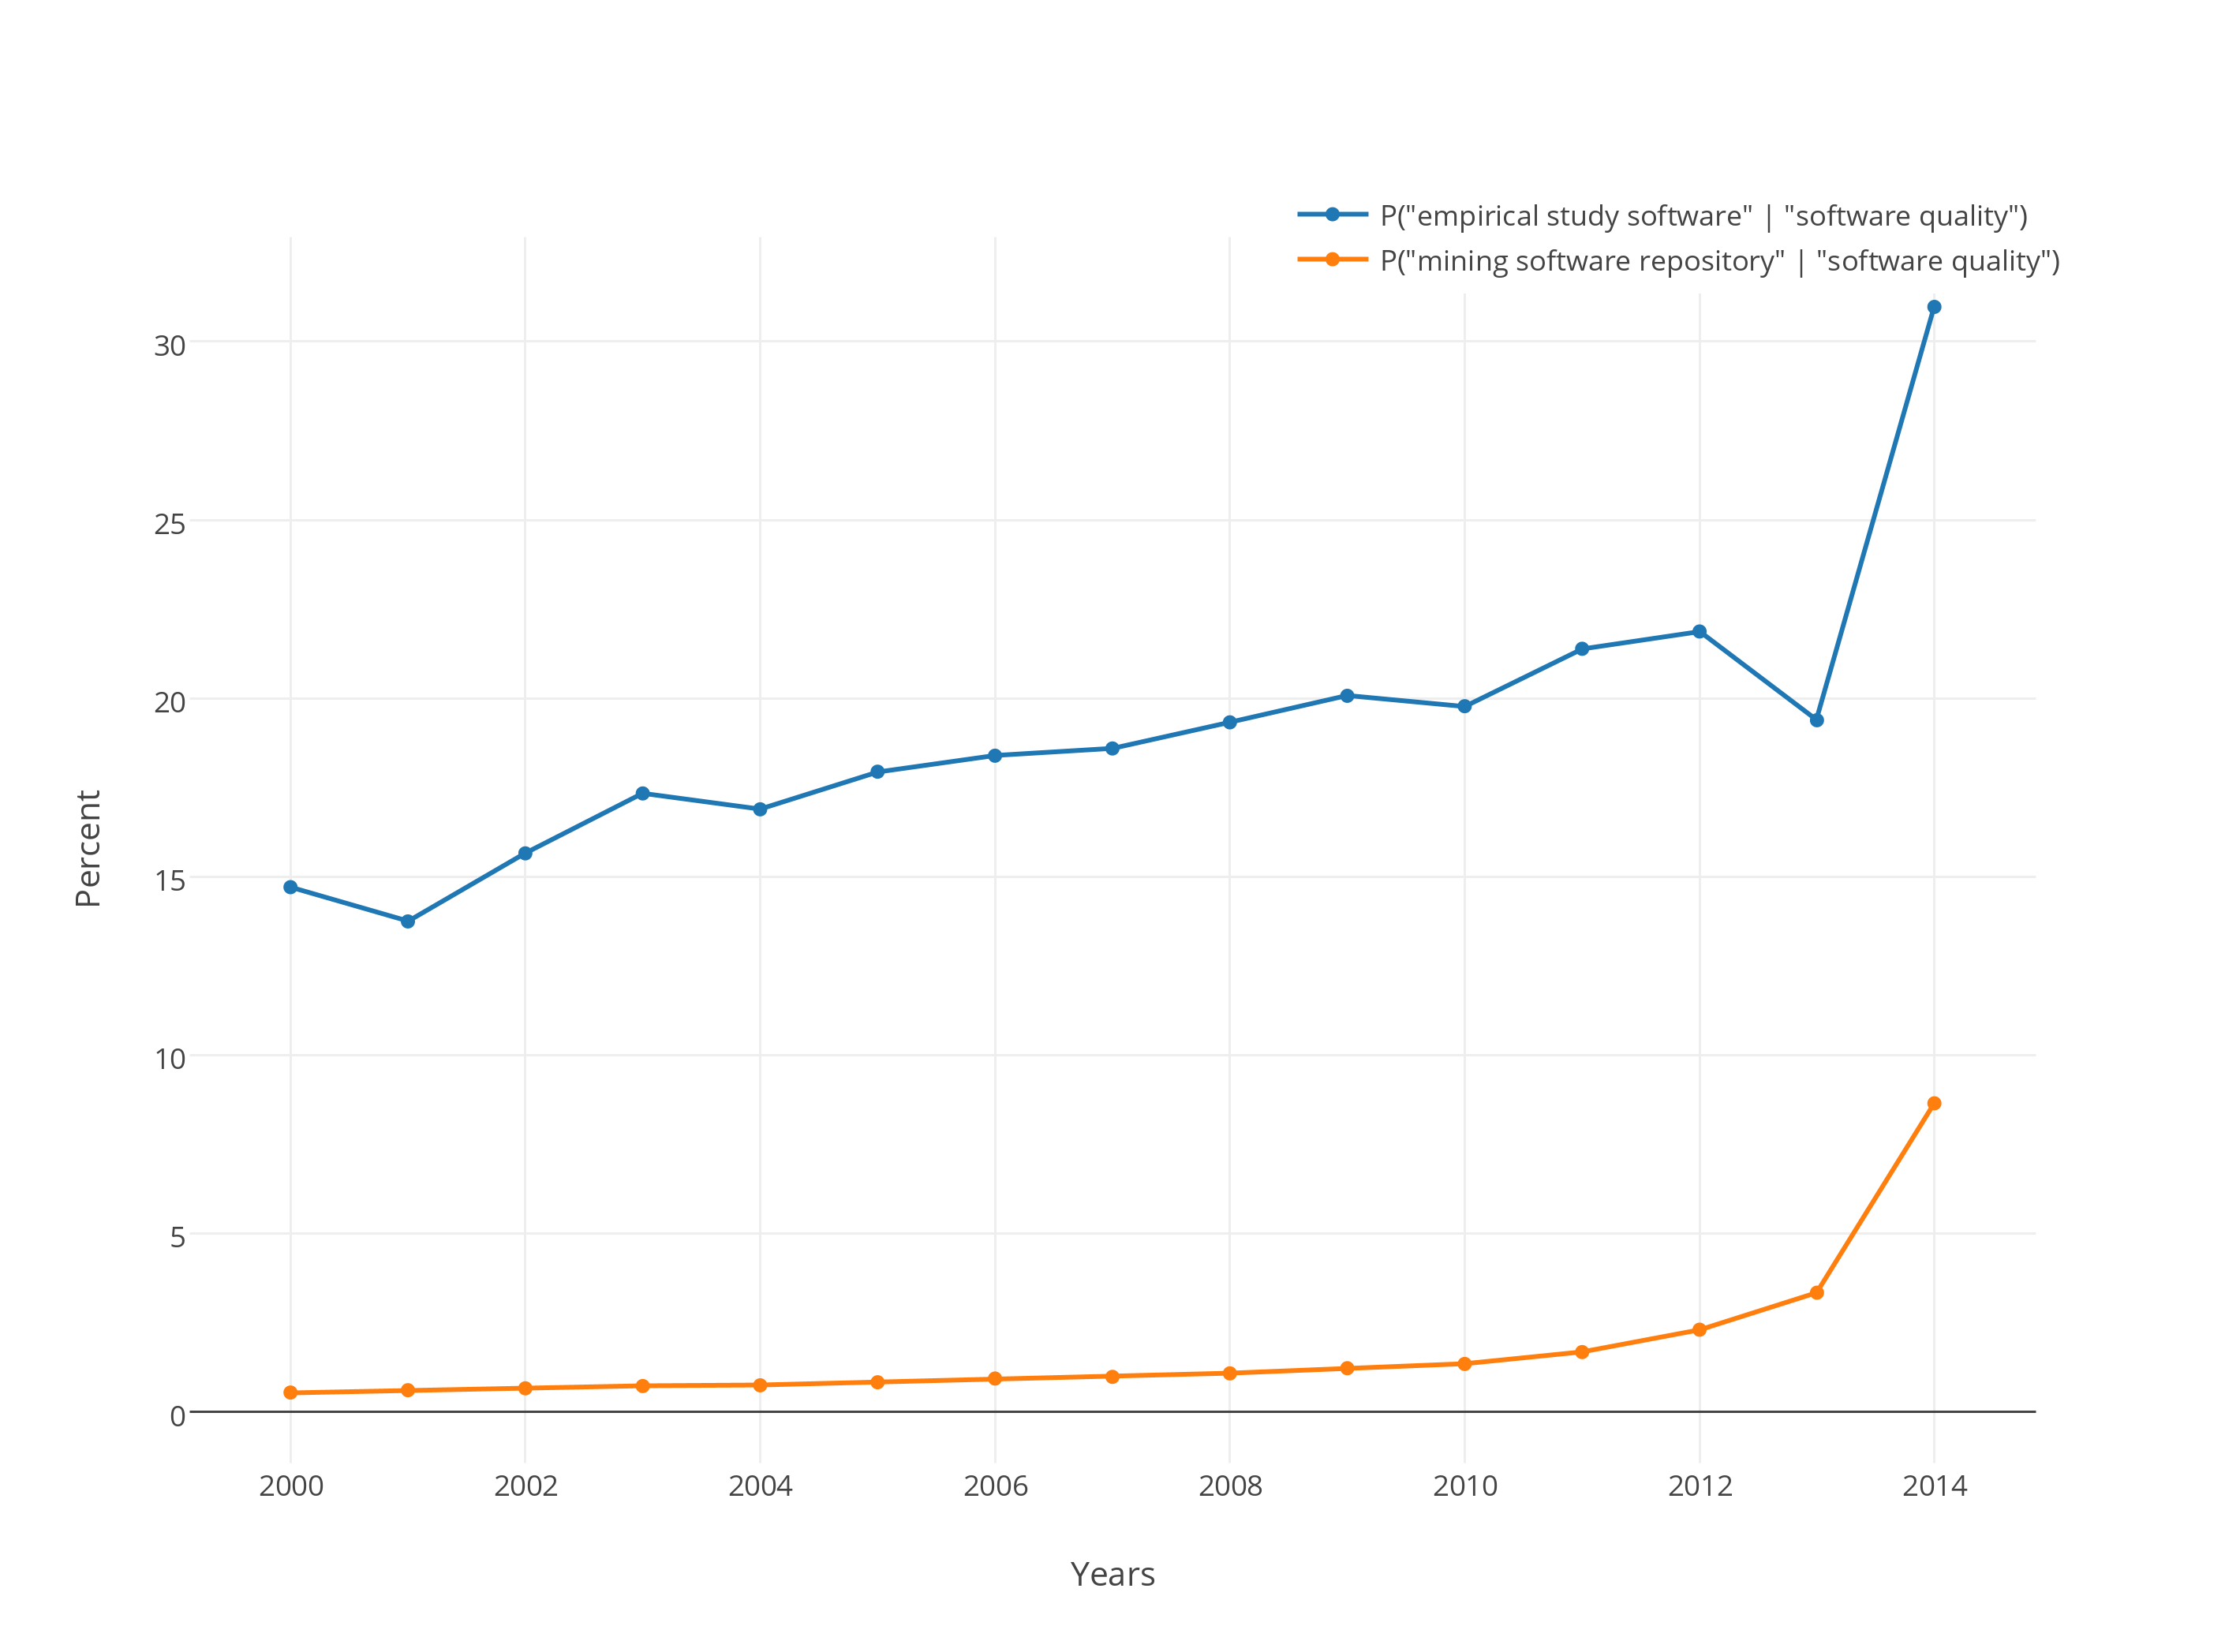
\includegraphics[scale=0.7]{media/scholar.png}
	    \caption{Proportion of papers containing ``Empirical Study'' or ``Mining software repository'' with regards to the paper in Software quality indexed by Google Scholar	\label{fig:scholar}}
	\end{figure}

	\item {\bf Problem 2}: The literature contains numerous papers about tools that improve the overall software quality with static \cite{Dangel2000, burn2003checkstyle, Hovemeyer2007, Moha2010} and dynamic \cite{Nayrolles,Nayrolles2013a,Palma2013} analysis. To the best of our knowledge approaches leveraging other sources to improve quality or efficiency mostly rely on web-search \cite{Brandt2009,Rahman2013,Montandon2013}.

	\item {\bf Problem 3}: There is no approach that supports the natural language search and comparison of issues, source code and tasks regardless of the project, repository, revision and issue management system and programming language. Such an approach could dramatically transform software engineering processes. Moreover, the data contained in these repositories lack a taxonomy, as for clone detection \cite{CoryKapser}, to classify the research.
\end{itemize}

\subsection{Research Challenges\label{sec:challenges}}

\begin{itemize}
	\item {\bf Challenge 1} : Issues \& projects and revision systems are plenty and they all have specific processes and limitations. Mining them all in order to have a representative model is challenging. Despite the parsing aspect, terabytes of new data are generated every day thus, storing and accessing to these data in reasonable time will require innovations in high density nosql databases \cite{Nayrolles2014b} and web servers \cite{Nayrolles2013b}. Moreover, creating the relationship between both systems is still an open issue as discussed in sections \ref{sec:issue-tracking} and \ref{rel:issue-rela}.

	\item {\bf Challenge 2}: Providing code samples broke down to the right level, at the right time in order to solve a problem  or improve the current code in terms of quality, performances or reliability during a programming session will force us to improve current approaches of source code transformation and normalization \cite{Cordy2006a, Cordy2006, Roy2008, Cordy2011}.
\end{itemize}

\subsection{Scope of the research \label{sec:scope}}

The area of this research is to improve the processes of software engineering by providing contextual information, in order to improve the quality, the performance, the reliability of a given code during a programming session. These contextual information will come from the mining issue \& project and revision systems. Hence, we will not define what are the good or bad practices to improve the quality, the performance, the reliability of a given code but rely on the mined data.

\subsection{Thesis contributions\label{sec:objective-thesis}}

Figure \ref{fig:proposal} depicts our proposed solution for fulfilling our objectives.
First of all, an end-user (team member) will report an issue (open a task) in one the organization issues \& project management system. This can be done in $Sourceforge$, $Bugzilla$, $JIRA$ or $Github$ which are the systems we want to support first as described in section \ref{sec:bug-provider}.

\begin{figure}[h!]
	\centering
	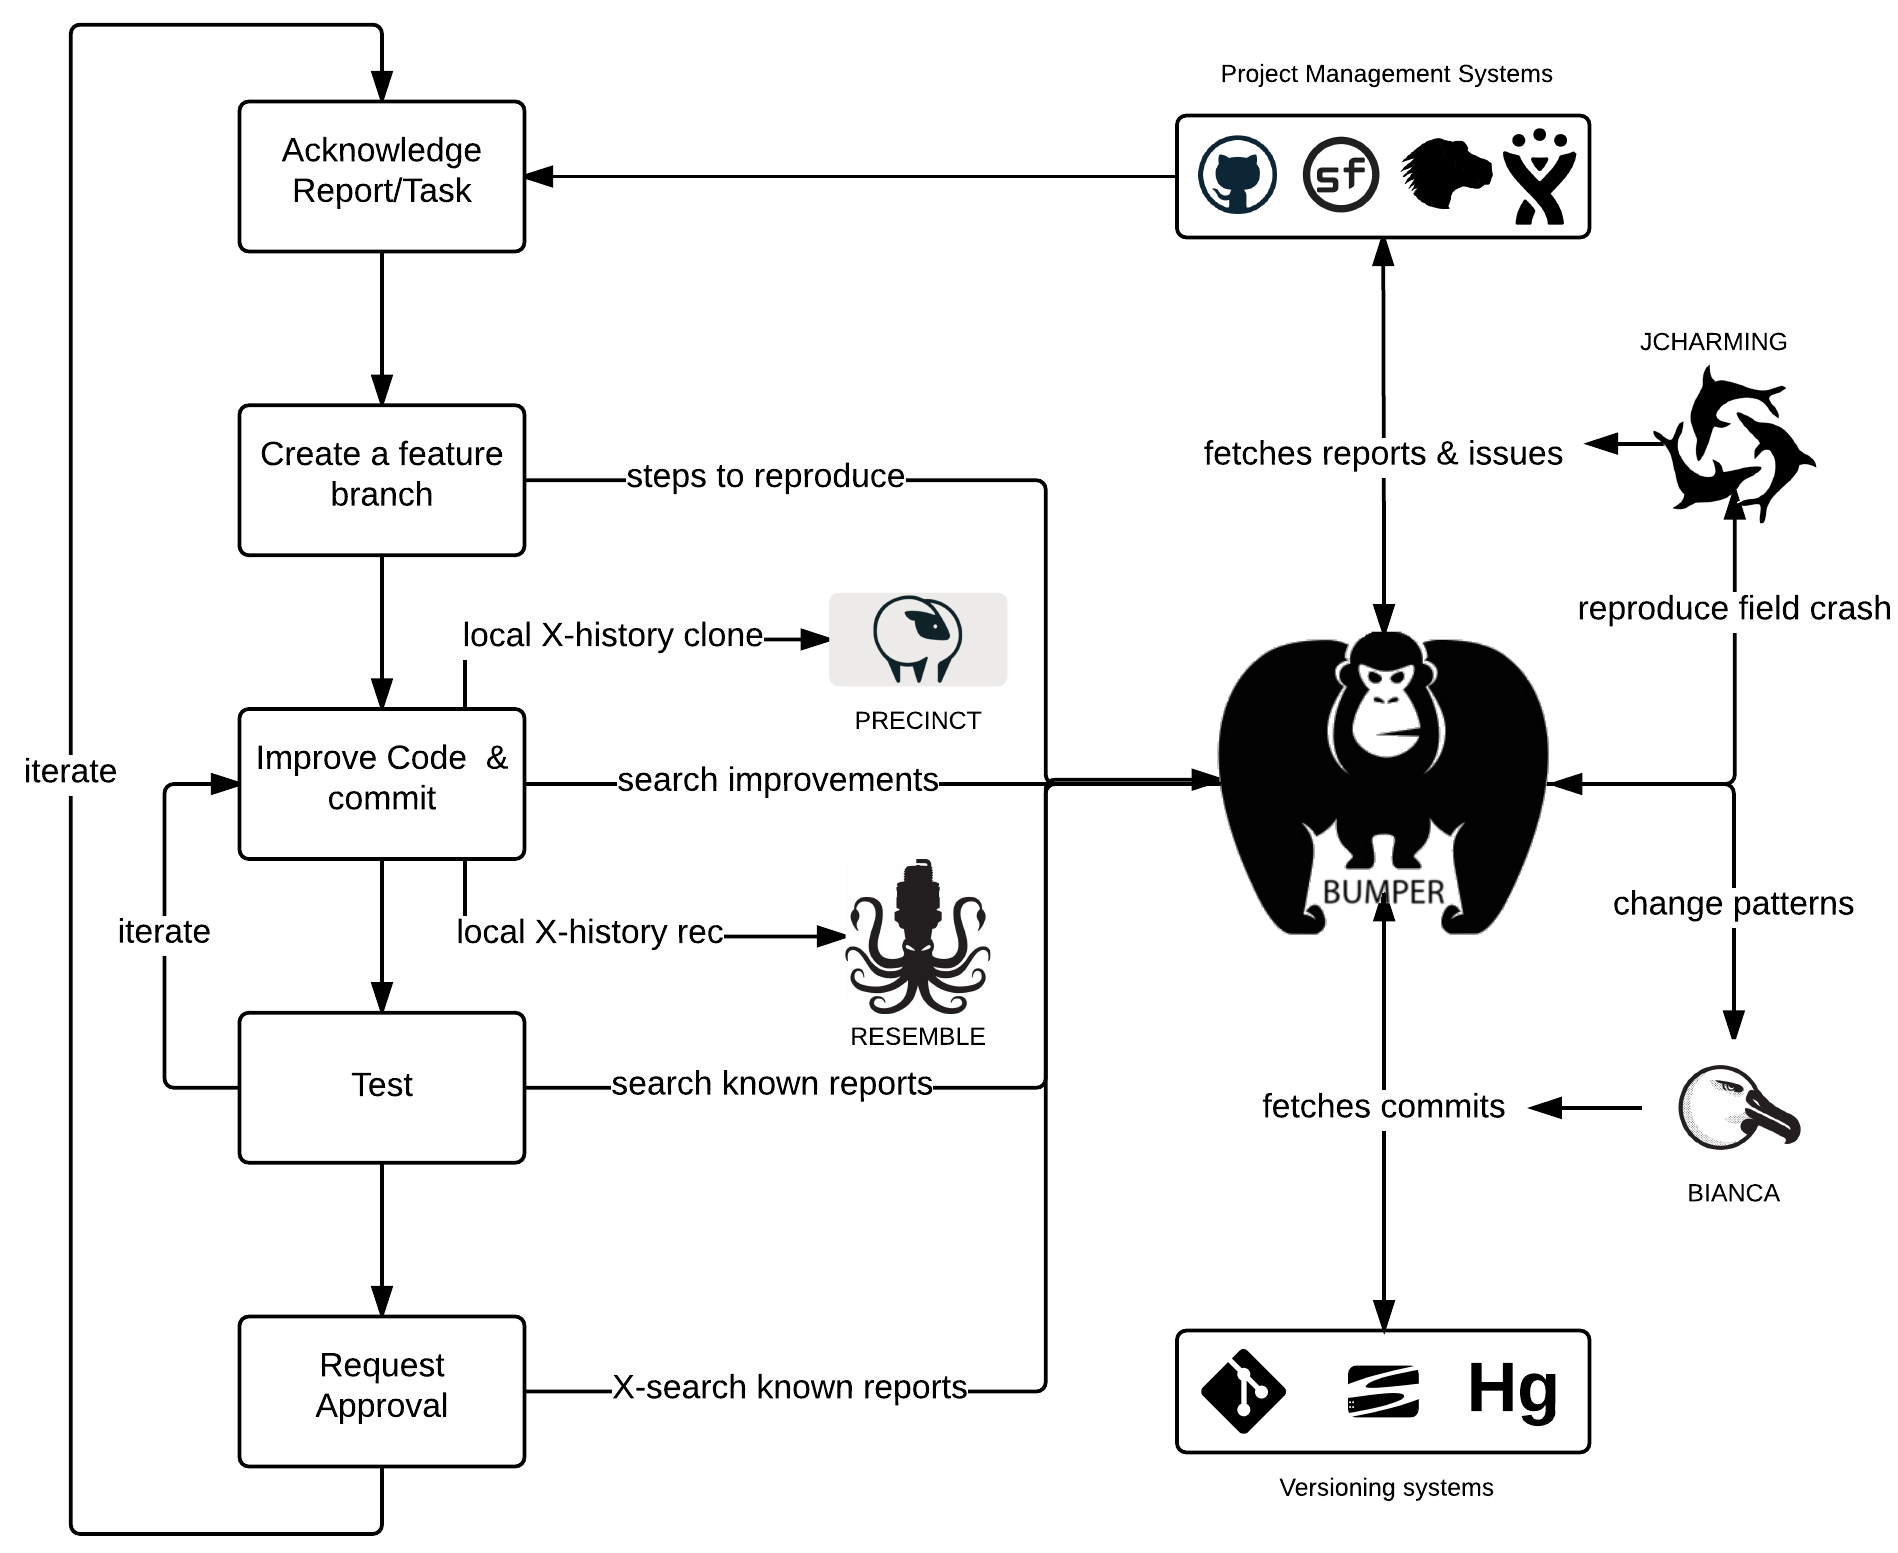
\includegraphics[scale=0.9]{media/proposal.png}
	\caption{Proposed Architecture}
	\label{fig:proposal}
\end{figure}


Issues (tasks) are  mapped with their fixes (implementations) inside {\tt BUMPER} (BUg MetarePository for dEvelopers and Researchers). The source code is fetched from the supported version system: $Git$, $Svn$, $Mercurial$ presented in section \ref{sec:version-control}.
{\tt BUMPER} is a meta-repository that makes issues, tasks and related source code searchable using natural language  (in opposition to structured query language).
When an issue is reported, {\tt JCHARMING} (Java CrasH Automatic Reproduction by directed Model checkING) will fetch the content of the issue and try to create a scenario to reproduce the on-field crash. In case of success, the developer assigned to this issue will be notified and the scenario stored in {\tt BUMPER}.
The developer assigned to the task or the issue will modify the code and, in real time, very much like intellisense or auto-completion in modern IDE, {\tt RESEMBLE} (REcommendation System based on cochangE Mining at Block LEvel) will propose improvements or follow up on the developer's code using the decades of history stored in {\tt BUMPER}. Once s/he is done, s/he submit a commit, patch or diff to the version system.
However, before s/he allowed to do so, {\tt BIANCA} (Bug Insertion ANticipation by Clone Analysis at commit time) will kick in and query {\tt BUMPER} looking for similar modifications in other projects and even other programming languages that led to the insertion of a defect in order to warn the user about potential hazardous code.


The bug taxonomy required to build {\tt BUMPER}, {\tt BUMPER} itself, {\tt JCHARMING}, {\tt RESSEMBLE} and {\tt BIANCA} are presented in sections \ref{sec:taxo}, \ref{sec:BUMPER}, \ref{sec:JCHARMING}, \ref{sec:RESEMBLE} and \ref{sec:BIANCA}, respectively. In addition, we list parts that have been published in peer-reviewed conferences in section \ref{sec:current-state} and our publication plan in \ref{sec:publication-plan}.

As a motivating example, we draft the following scenario. Table \ref{tab:bumper-hypo} presents hypothetical data stored in {\tt BUMPER} in terms of sequence \#id, sequence of code blocks, a flag to know if a said sequence introduced an issue in a given system and step to reproduce the issue if any.

\begin{table}[h!]
\centering
\begin{tabular}{c|c|c|c|c}
Seq \#ID & Language \#ID & Blocks & Root of Issue & Steps to reproduce \\ \hline \hline
1        & 1             & A-A-B-C-A-A   & Yes  & E-F-G         \\
2        & 1             & A-A-B-C       & No   & -         \\
3        & 2             & D-E-A-C       & No &  - \\ \hline \hline
\end{tabular}
\caption{Hypothetical {\tt BUMPER} data}
\label{tab:bumper-hypo}
\end{table}

During a programming session, let's assume that a developer has implemented $A-B-C$, then {\tt RESEMBLE} will recommends to transform the current code to $A-A-B-C$ as it seems to be the right thing to do.
If the developer follows {\tt RESEMBLE} recommendation and then adds another two $A$s, the sequence is now $A-A-B-C-A-A$.
If the developer commit its changes, {\tt BIANCA} will raise a warning saying that this sequence is known to be the root of an issue and invite the developer to execute the steps $E-F-G$ -- that were produced by {\tt JCHARMING} -- in order to see if s/he did introduce a defect. Moreover, {\tt BIANCA} will take the time to compare $A-A-B-C-A-A$ and $D-E-A-C$ using our normalization algorithms even if they are not in the same programming language.
Finally, when a new issue is submitted, {\tt BUMPER} indexes it and {\tt JCHARMING} tries to reproduce it and update the step to reproduce part of {\tt BUMPER}.

We can envision the potential of such a system and its complexity, knowing that it would contain millions of issues, hundreds of thousand projects, dozens of programming languages and will help developers leveraging the knowledge of other developers.

To summarize this thesis have four main contributions:

\begin{itemize}
	\item To provide a taxonomy of software issues to classify the research.
	\item To propose approaches to aggregate as many issues and revisions systems as possible.
	\item To propose approaches to reproduce field crashes in a lab environment using the issue content.
	\item To propose a context-aware IDE that will improve day-to-day programming session with concise and appropriate code samples.
\end{itemize}

\section{Outline\label{sec:outline}}
